\documentclass[11pt]{article}
\usepackage[margin=1in]{geometry}
\usepackage{graphicx}
\usepackage{booktabs}
\usepackage{float}
\usepackage{hyperref}
\usepackage{enumitem}
\hypersetup{colorlinks=true, linkcolor=blue, urlcolor=blue}
\setlength{\parindent}{0pt}
\setlength{\parskip}{0.6em}

\title{OLMo2 1B degeneration progression (50 prompts)}
\author{}
\date{2026-04-05 01:37 UTC}

\begin{document}
\maketitle

\section*{Stage Map}
\begin{itemize}[leftmargin=1.5em]
\item \textbf{Base}: \texttt{allenai/OLMo-2-0425-1B}
\item \textbf{SFT}: \texttt{allenai/OLMo-2-0425-1B-SFT}
\item \textbf{RLVR1}: \texttt{allenai/OLMo-2-0425-1B-RLVR1}
\item \textbf{Instruct}: \texttt{allenai/OLMo-2-0425-1B-Instruct}
\end{itemize}

\section*{Shared Contract}
This progression bundle compares multiple checkpoints under one rollout-statistics contract. The stage summaries were validated to share temperature, number of generations, max token budget, max model length, dtype, trust-remote-code flag, loop detector, and tracked statistics before plotting the progression.

\section*{Headline Read}
Average loop fraction moves from 40.8\% on Base to 5.3\% on Instruct.

Average max-length-hit fraction moves from 61.9\% on Base to 7.6\% on Instruct.

MATH-500: loop fraction moves from 37.8\% (Base) to 2.4\% (Instruct); max-length-hit fraction moves from 42.2\% to 3.0\%.

AIME 2024/2025: loop fraction moves from 44.8\% (Base) to 5.4\% (Instruct); max-length-hit fraction moves from 48.0\% to 7.2\%.

GPQA Diamond: loop fraction moves from 51.2\% (Base) to 4.2\% (Instruct); max-length-hit fraction moves from 61.6\% to 8.8\%.

MMLU-Pro: loop fraction moves from 47.0\% (Base) to 14.0\% (Instruct); max-length-hit fraction moves from 62.6\% to 18.6\%.

\begin{figure}[H]
\centering
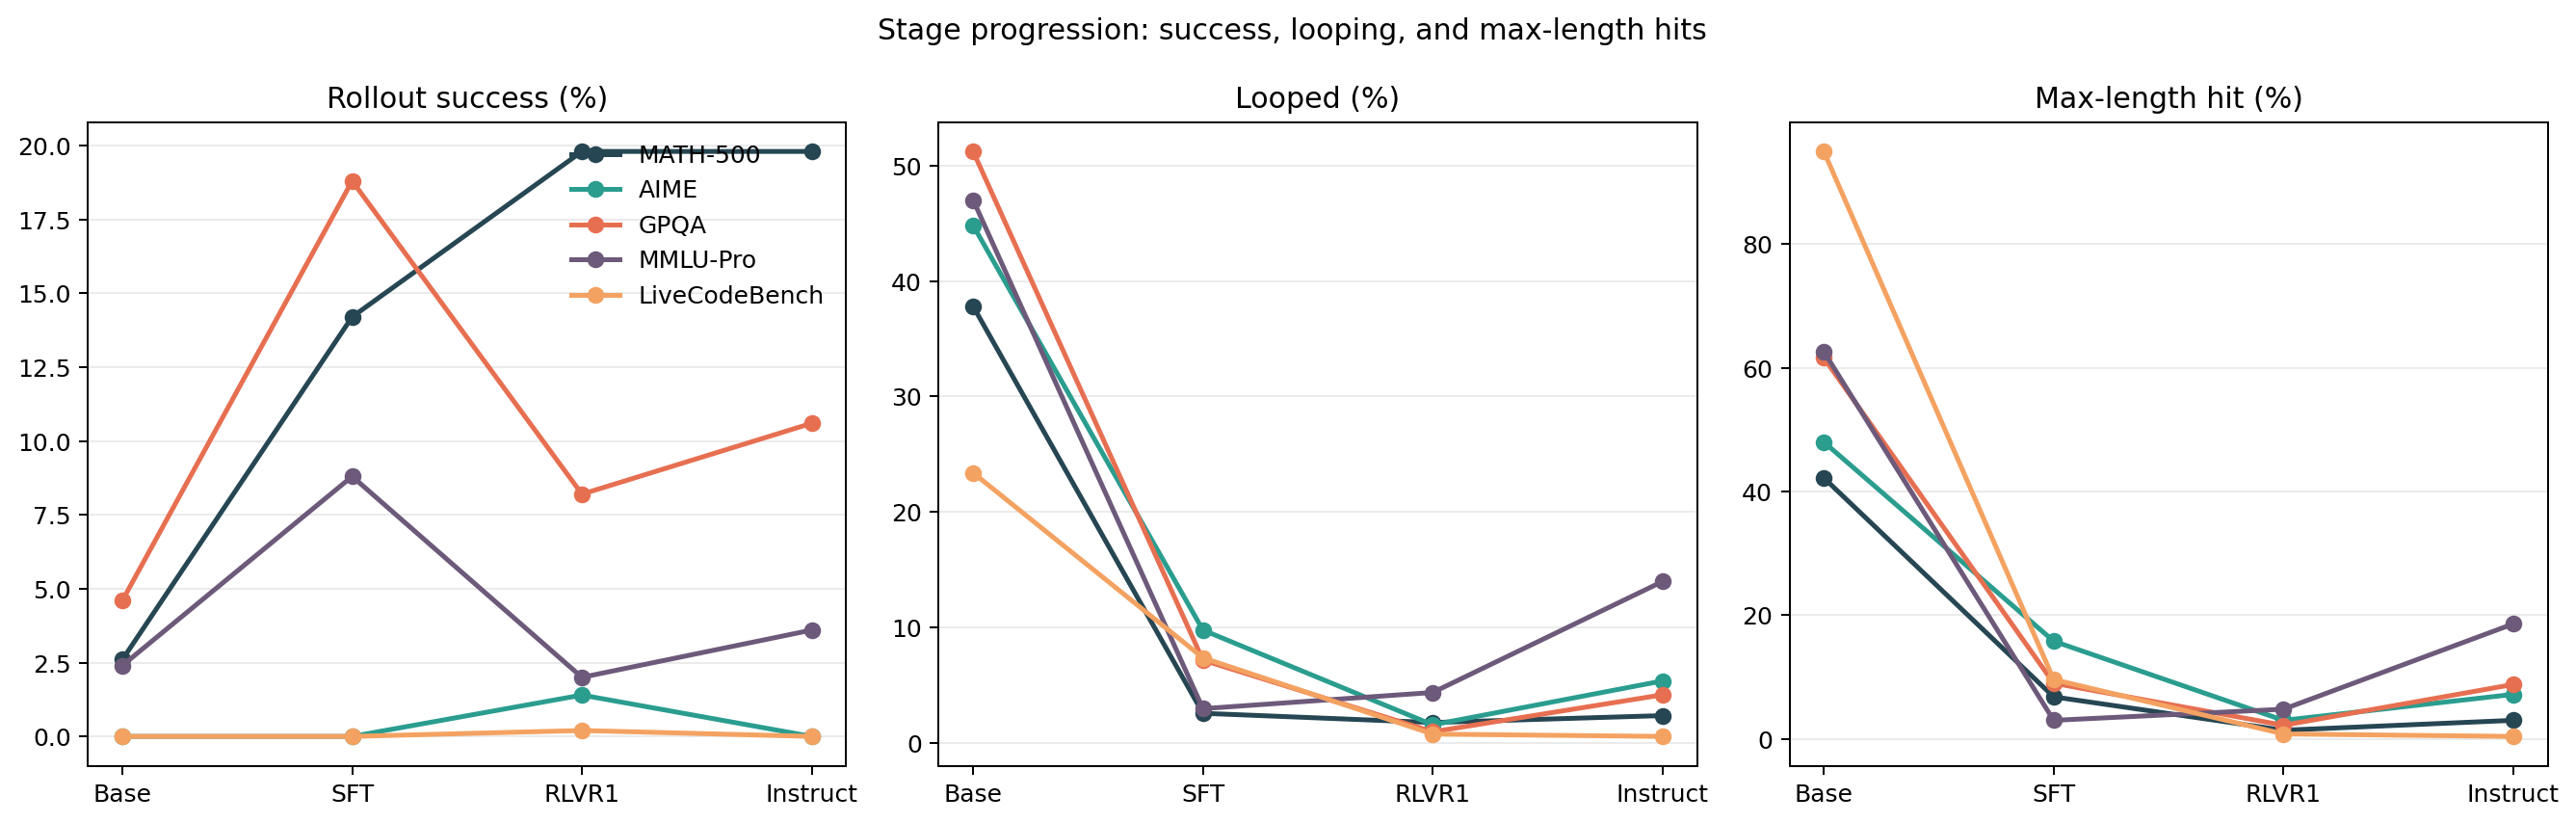
\includegraphics[width=\textwidth]{figures/progression_rates.png}
\caption{Progression of rollout success, loop rate, and max-length-hit rate across stages, broken out by dataset.}
\end{figure}

\begin{figure}[H]
\centering
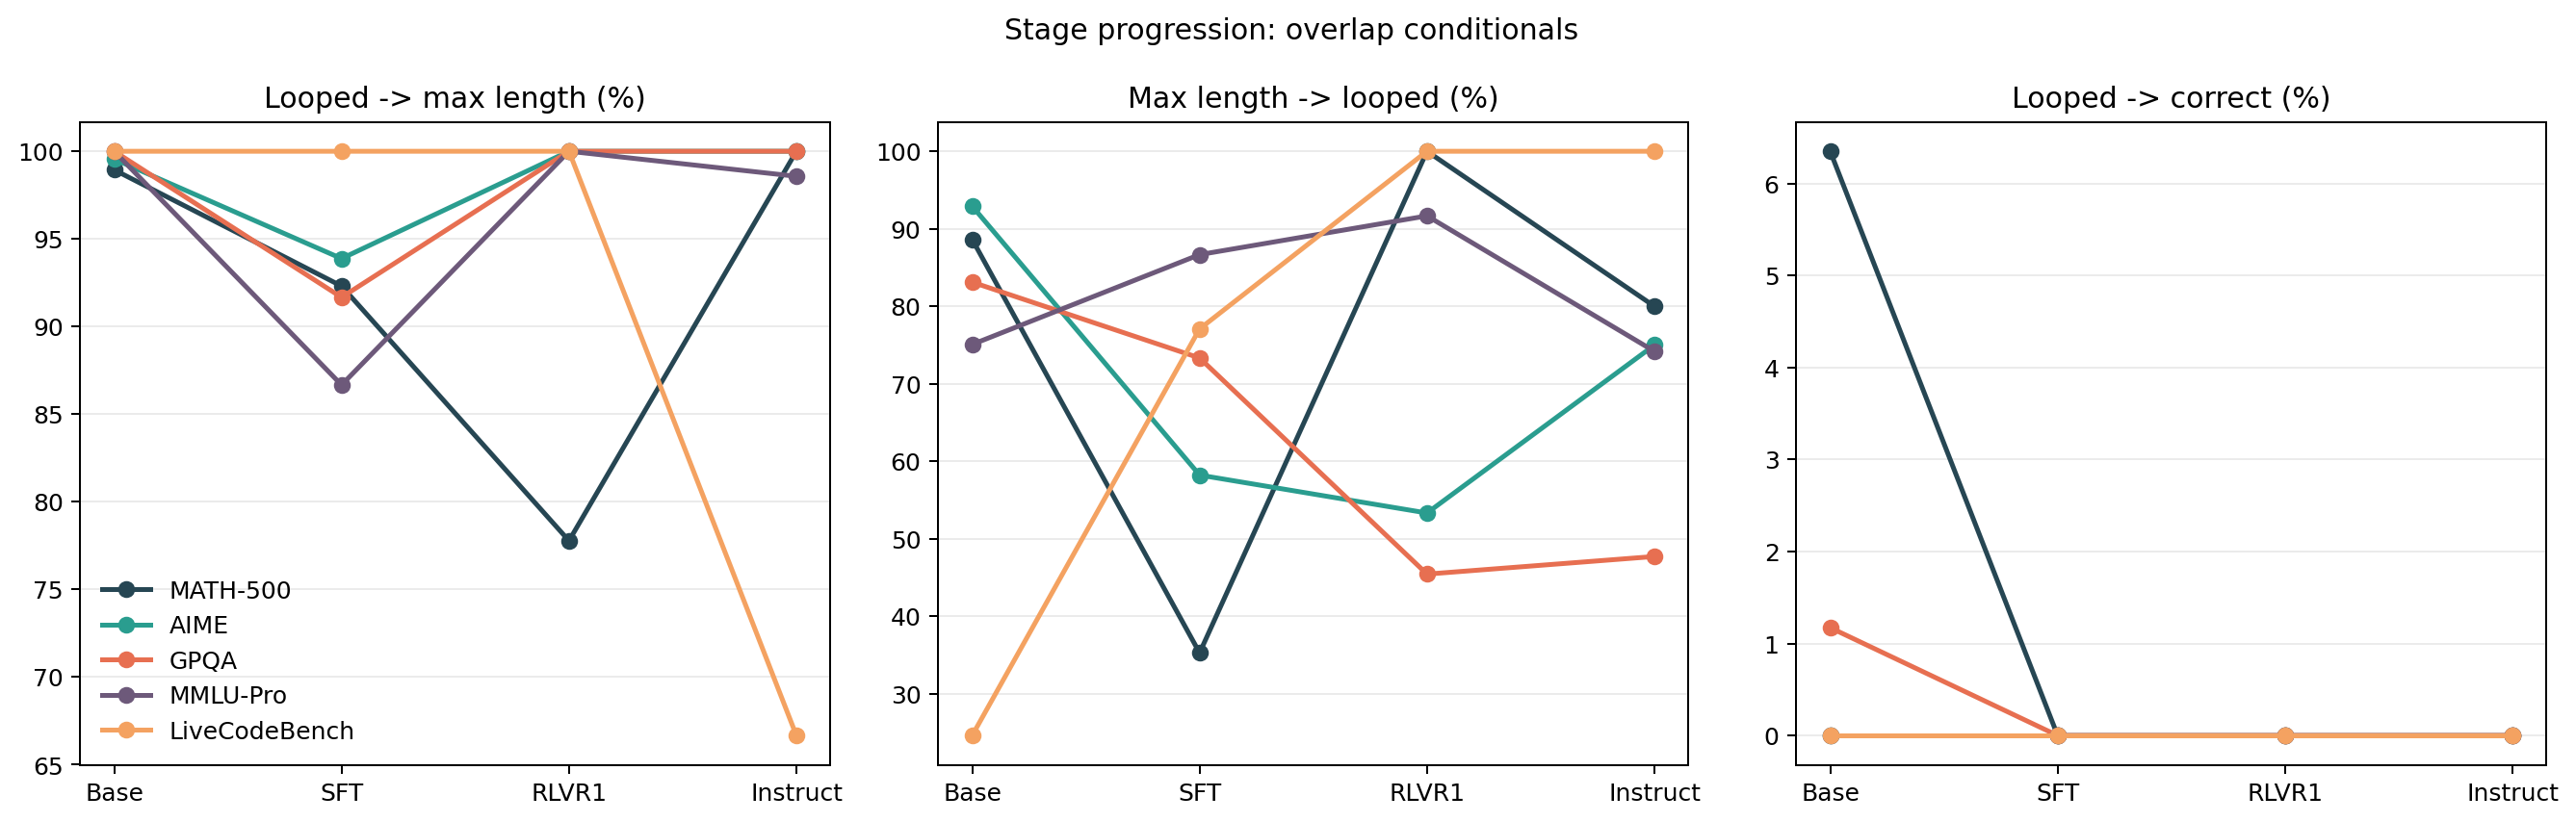
\includegraphics[width=\textwidth]{figures/progression_overlap.png}
\caption{Progression of overlap conditionals across stages, broken out by dataset.}
\end{figure}

\begin{figure}[H]
\centering
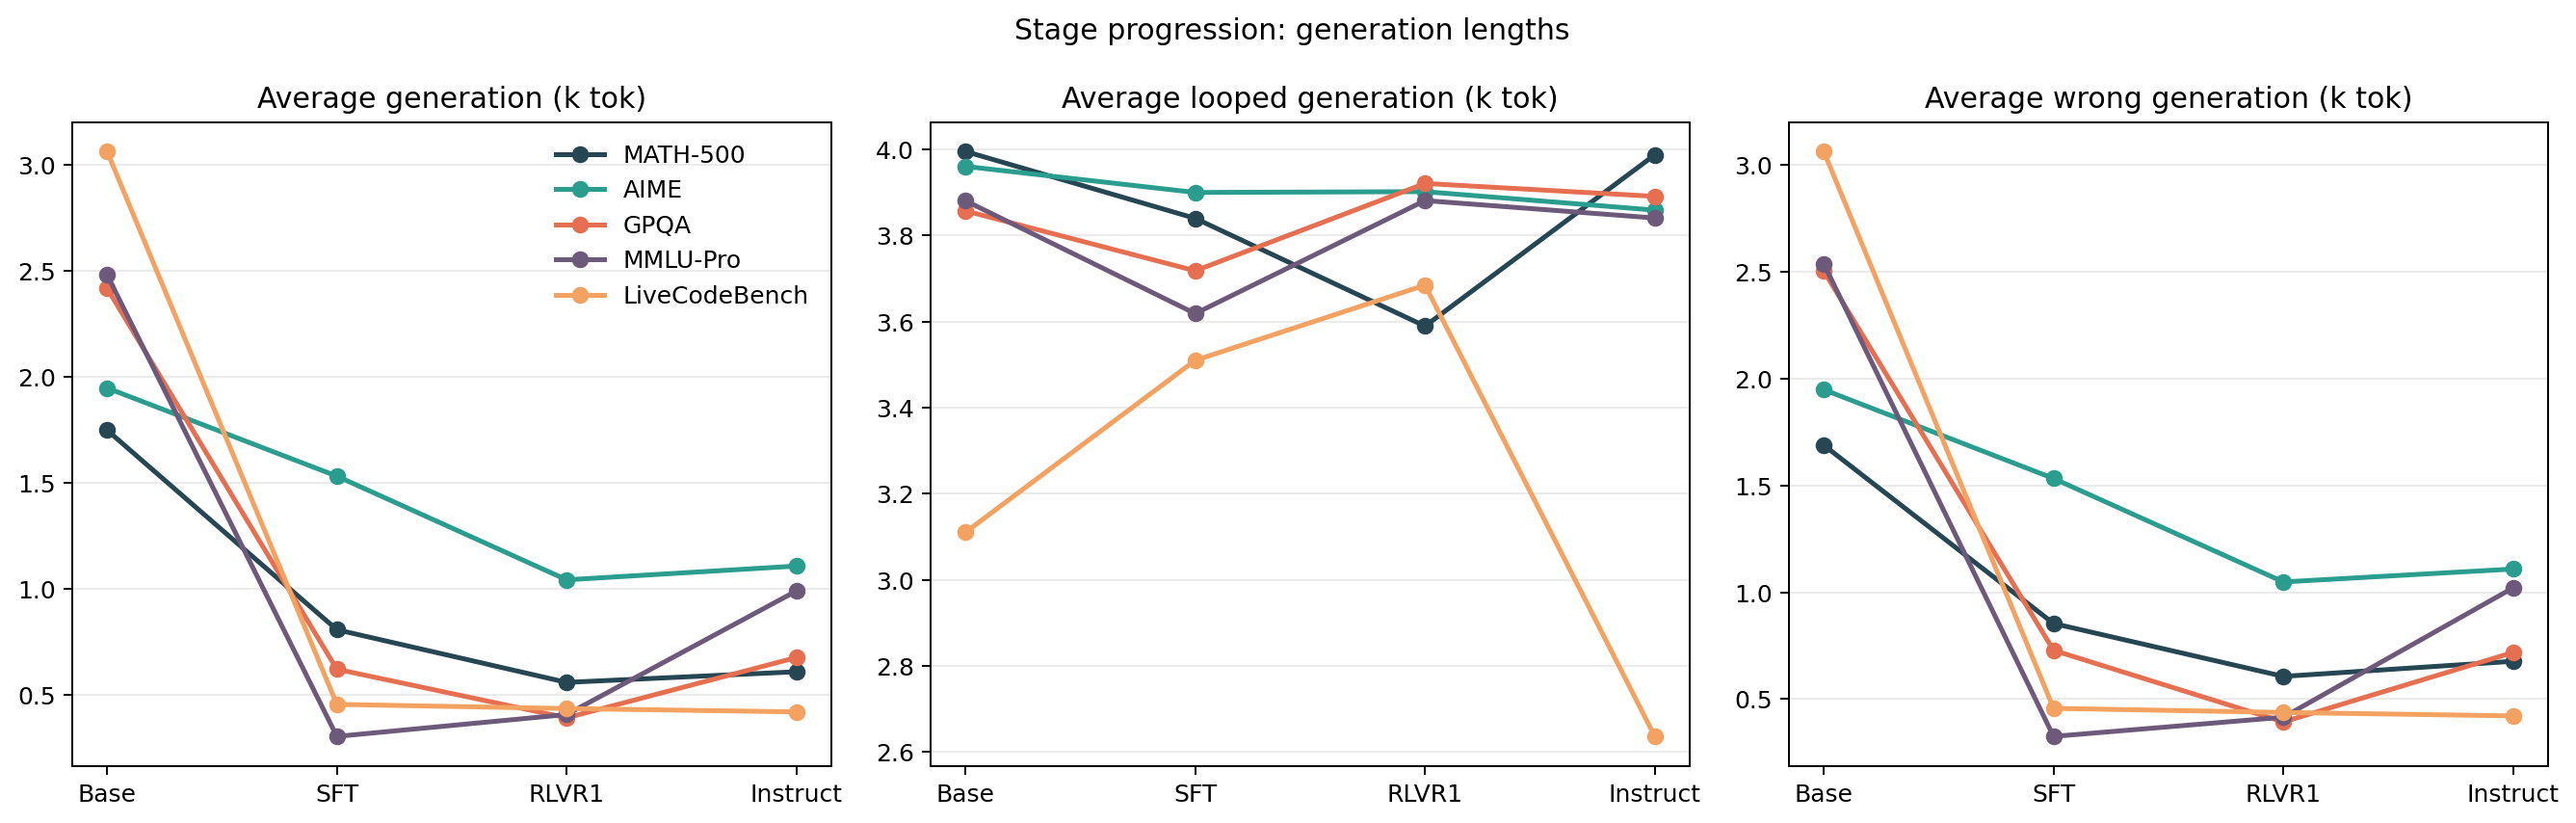
\includegraphics[width=\textwidth]{figures/progression_lengths.png}
\caption{Progression of generation-length statistics across stages, broken out by dataset.}
\end{figure}

\begin{figure}[H]
\centering
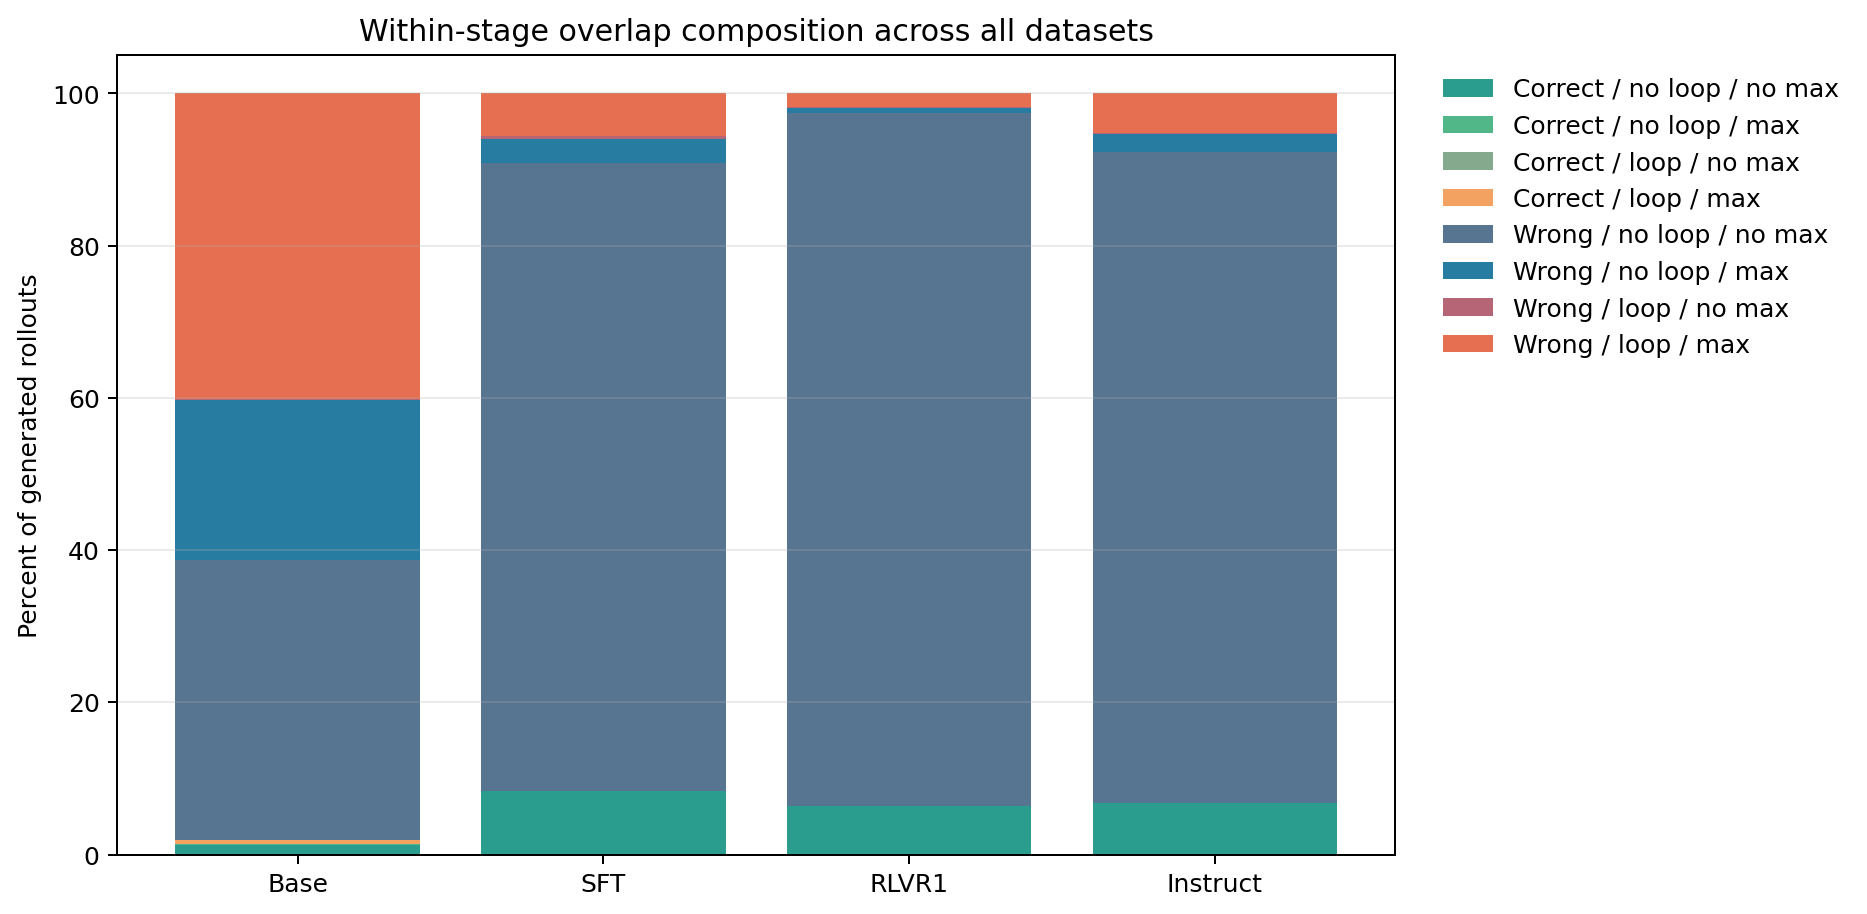
\includegraphics[width=\textwidth]{figures/stage_overlap_composition.png}
\caption{Within-stage overlap composition aggregated across all datasets. This uses the saved raw counts to decompose generated rollouts by correctness, loop status, and max-length-hit status.}
\end{figure}

\begin{figure}[H]
\centering
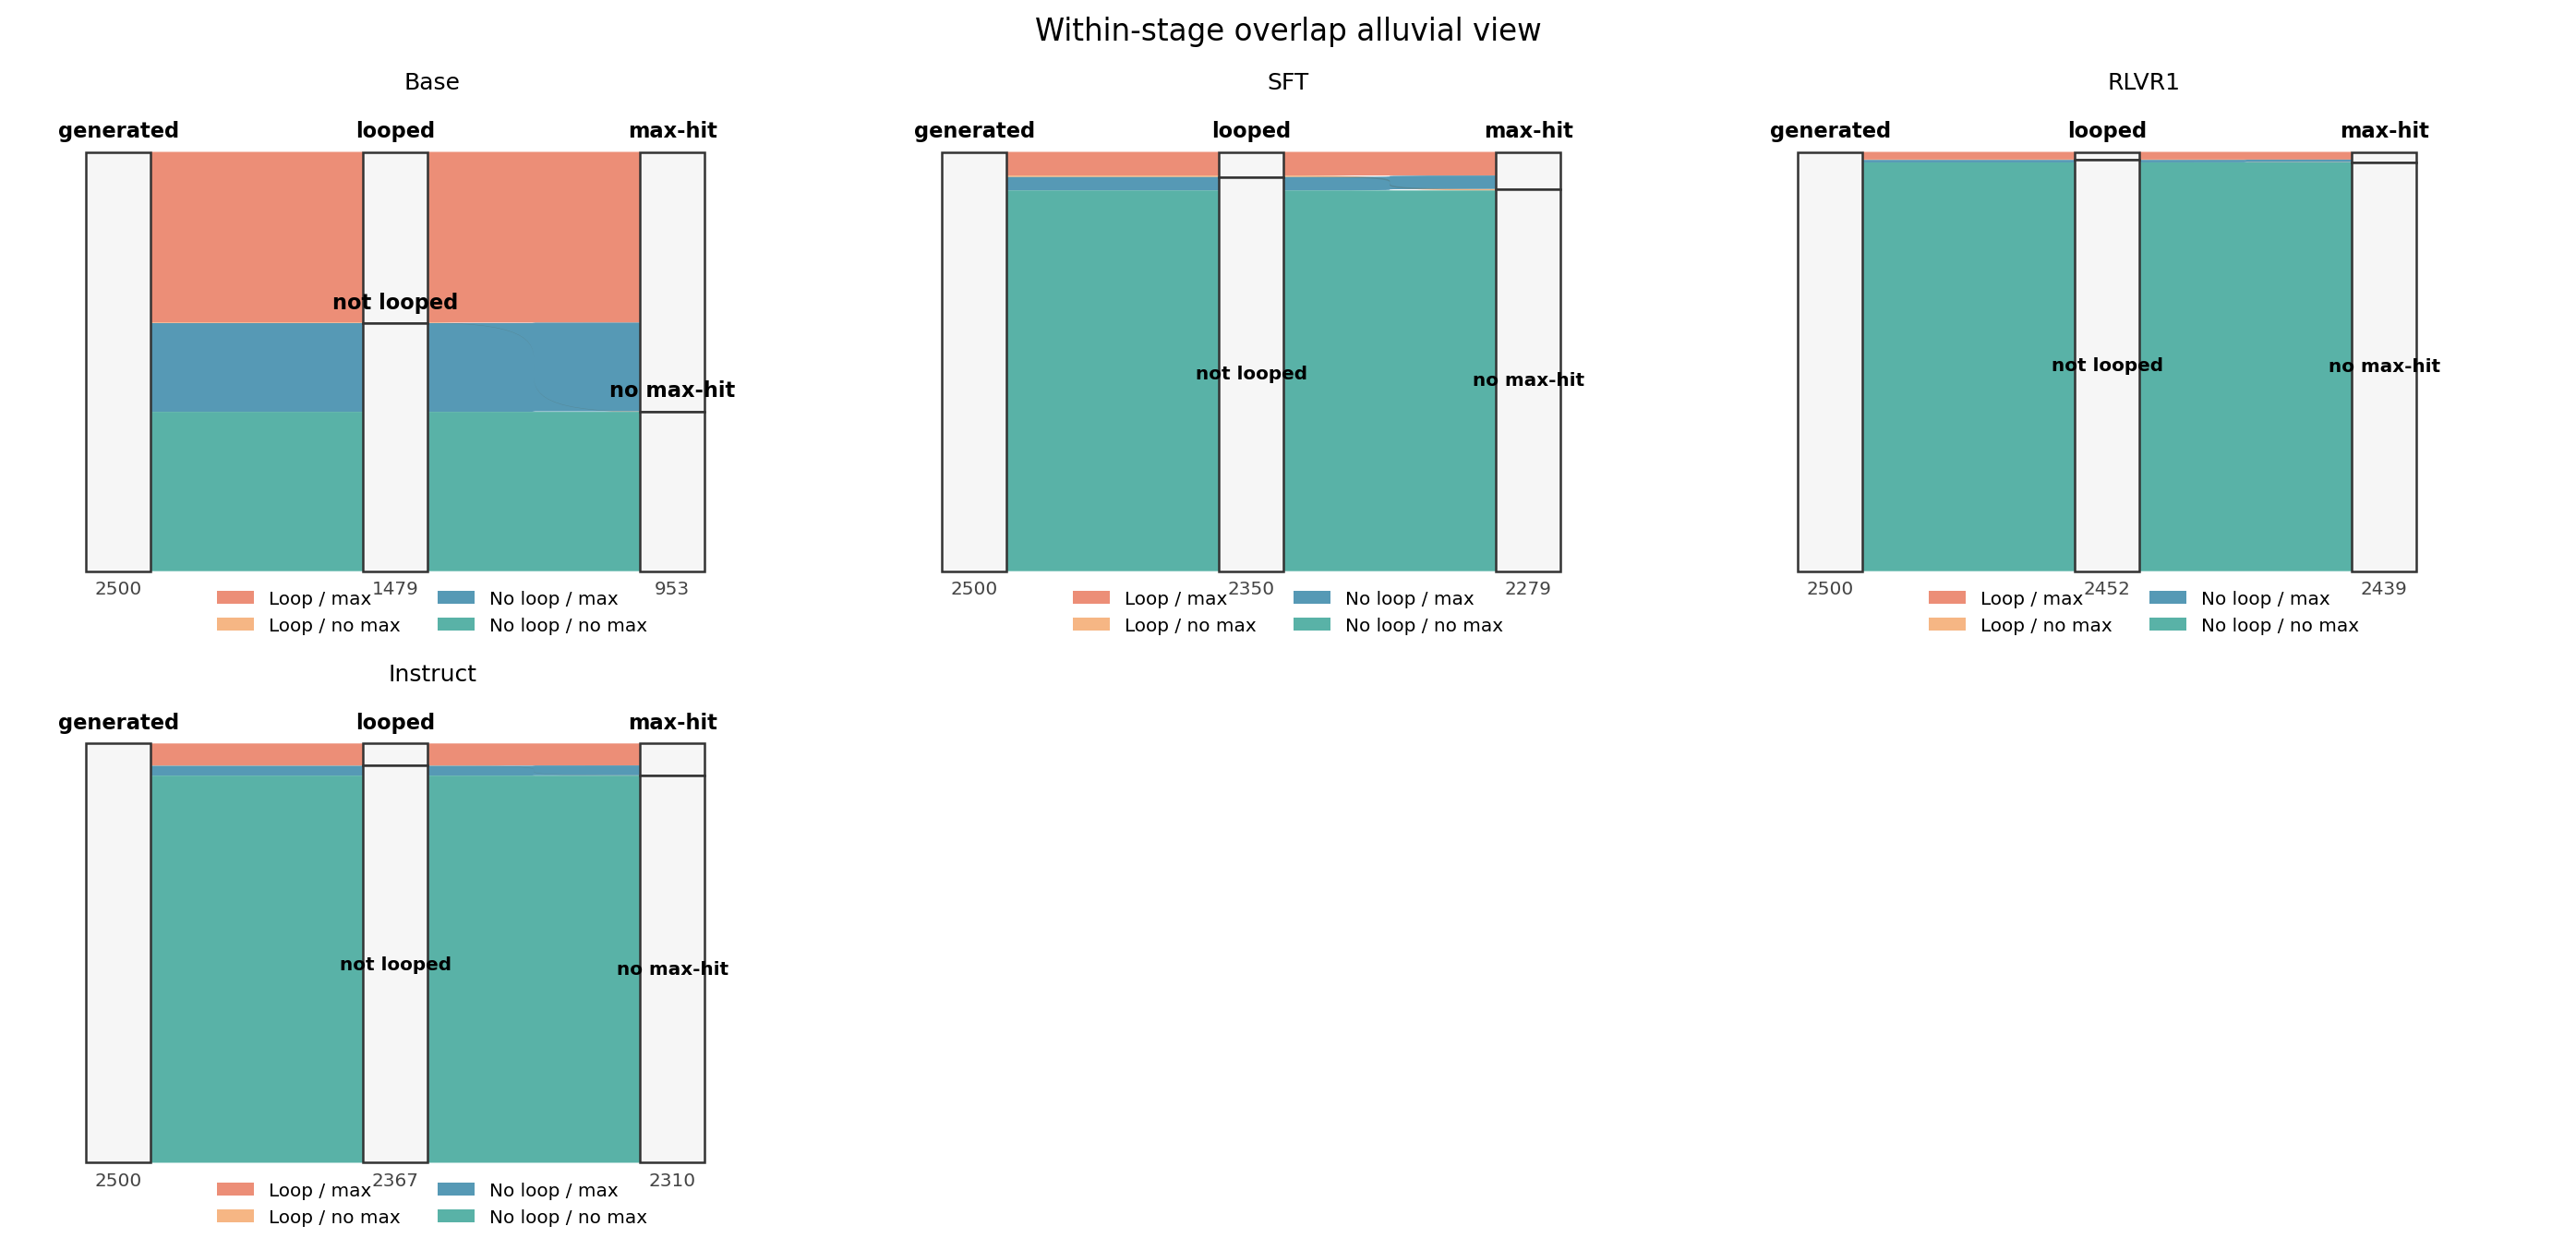
\includegraphics[width=\textwidth]{figures/stage_overlap_sankey.png}
\caption{Within-stage alluvial view of the overlap structure. Each stage shows how generated rollouts split into looped versus non-looped branches and then into max-length-hit versus non-max-length-hit branches.}
\end{figure}

\section*{Interpretation}
The progression figures answer the exact object of the note: where the degenerate-rollout regime enters the model family under a fixed rollout contract. The line plots are the stage comparison surface; the overlap-composition panel makes the within-stage structure visible without collapsing everything to one scalar rate. If the loop and max-length-hit curves are near-zero in the base stage and then rise sharply after SFT or RLVR, that is direct evidence for a stage-linked introduction of degenerate rollouts. If they are already substantial in the base model, the hypothesis weakens.

\end{document}
